% Filename  : samplepaper.tex
% Purpose   : A sample exam paper to demonstrate how to use the 'ditpaper'
%             TeX class.
% Author    : Emmet Caulfield
% Revision  : $Id: samplepaper.tex 2 2006-02-19 20:34:45Z emmet $
% Repository: $HeadURL: http://svn.netrogen.lan/tex-ditpaper/trunk/samplepaper.tex $
%

% 'nosolution' (default) and 'solution' toggle the inclusion of solutions
% in the output. The tag solution, below, is replaced by 'sed' 
% in the Makefile to cause both the paper and the solutions to be produced.
\documentclass[solution]{ditpaper}

\usepackage{graphicx}
\usepackage{multirow}
\usepackage{rotating}


% These must be set or bizarre defaults will be used:
\facility{Kevin Street, Dublin 8}
\course{BSc (Hons) in Computer Science}
\examcode{R228/406}
\stage{Stage 4}
\session{Supplemental Examinations 2010}
\title{Artificial Intelligence 2}
\examiners{Dr. John Kelleher\\
Dr. D. Lillis\\
Dr. I. Arana}
\examdate{}
\examtime{Duration: 2 Hours}
\instructions{Answer Question 1 (40 marks) \textbf{and}\par{} any 2 Other Questions (30 marks each).}

\begin{document}

% basic probability and machine learning experiments
\question
\begin{enumerate}
	\item Given the full joint distribution shown in Table \ref{tab:fjd}, calculate the following:
			\begin{table}[htb]
		\caption{Full joint distribution for a dentist visit}
		\begin{center}
		\begin{tabular}{c|c|c|c|c|}
		                          & \multicolumn{2}{c}{$toothache$} \vline & \multicolumn{2}{c}{$\lnot toothache$}  \vline \\
		\hline
		                          & $catch$ & $\lnot catch$ & $catch$ & $\lnot catch$ \\
		 $cavity$          & 0.108     & 0.012             & 0.072      & 0.008             \\
		 $\lnot cavity$ & 0.016     & 0.064             & 0.144      & 0.576             \\
		\end{tabular}
		\end{center}
		\label{tab:fjd}
		\end{table}%
	\begin{enumerate}
		\item $P(toothache)$
		\marks{5}
		\begin{answer}
		This asks for the probability that $Toothache$ is true. $P(toothache) = 0.108 + 0.012 + 0.016 + 0.064 = 0.2 $
		\end{answer}
		\item $\textbf{P}(Cavity)$
		\marks{5}
		\begin{answer}
		This asks for the vector of probability values for the random variable $Cavity$. It has two values, which we list in the order $\langle true , false \rangle$. First add up $P(cavity)=0.108 + 0.012 + 0.072 + 0.008 = 0.2.$ Then we have $textbf{P}(Cavity ) =\langle 0.2, 0.8\rangle$ . 
		\end{answer}
		\item $\textbf{P}(Toothache|cavity)$
		\marks{5}
		\begin{answer}
		This asks for the vector of probability values for $Toothache$, given that $Cavity$ is true. $textbf{P}(Toothache|cavity ) = \langle\frac{0.108 + .012}{0.2}, \frac{0.072 + 0.008}{0.2}\rangle = \langle 0.6, 0.4\rangle$ 
		\end{answer}
		\item $\textbf{P}(Cavity|toothache \lor catch)$
		\marks{5}
		\begin{answer}
		This asks for the vector of probability values for $Cavity$, given that either $Toothache$ or $Catch$ is true.\\
		Recall $P(a|b) = \frac{P(a \land b)}{P(b)} \rightarrow$ \\
		$\textbf{P}(Cavity|toothache \lor catch) =$\\
		 $\langle \frac{P(cavity \land (toothache \lor cavity))}{P(toothache \lor catch)}, \frac{P(\lnot cavity \land (toothache \lor cavity))}{P(toothache \lor catch)}\rangle$\\
		First compute $P(toothache \lor catch) = 0.108 + 0.012 + 0.016 + 0.064 + 0.072 + 0.144 = 0.416$. \\
		Then $\textbf{P}(Cavity | toothache \lor catch ) =$\\
		 $\langle \frac{0.108 + 0.012 + 0.072}{0.416}, \frac{0.016 + 0.064 + 0.144}{0.416}\rangle = \langle 0.4615, 0.5384\rangle$ \\
		\end{answer}
	\end{enumerate}		
		\item Describe the problems associated with measuring \textbf{classifier performance} using a single accuracy figure \textbf{and} describe a more appropriate alternative.
		\marks{20}
	\begin{answer}
		This is a discursive question so giving a precise answer is not appropriate. However, an answer to this question should describe how a single accuracy figure can hide a classifier's real performance. An example should be provided such as the following:
		
		\begin{itemize}
			\item Text cases: 1000
			\item Positive examples: 900
			\item Negative examples: 100
		\end{itemize}
		
		Assuming the classifier always classifies positively then its accuracy on the given text set would be 90\% which is not an accurate reflection of the classifiers performance.
		
		 The most obvious alternative would be to describe the use of \textbf{specificity}, \textbf{sensitivity} and \textbf{precision} along with a \textbf{confusion matrix}. Students should explain how a confusion matrix can be use as follows:
		 
				\begin{tabular}{|c|c|c|c|}
				\multicolumn{2}{|c|}{Classifier Results} & & \\
				Class A (yes) & Class B (no) &  & \\
				\hline
				Correct & $F_{n}$ & Class A (yes) & \multirow{2}{*}{Expected Results}\\
				$F_{p}$ & Correct & Class B (no) & \\
				\end{tabular}
		
		And finally it is expected that the students would describe specificity, sensitivity and precision as follows:
		
		$sensitivity = \frac{t_{pos}}{pos}$
		$specificity = \frac{t_{neg}}{neg}$
		$precision = \frac{t_{pos}}{t_{pos}+f_{pos}}$
		
	\end{answer}
\end{enumerate}

\newpage

%Q2 30 marks
% bayesian networks & reasoning under uncertainty
% aima chapters 14, 20 + Mitchell chapter 6 
% bayesian learning 
\question
\begin{enumerate}
		\item  In you local power station, there is an alarm that senses when a temperature gauge exceeds a given threshold. The gauge measures the temperature of the core of the power station. Consider the Boolean variables $A$ (alarm sounds), $F_A$ (alarm is faulty), and $F_G$ (gauge is faulty); and multivalued nodes $G$ (gauge reading) and $T$ (actual core temperature).
		\begin{enumerate}
			\item Draw a Bayesian network for this domain, given that the gauge is more likely to fail when the core temperature gets too high.
			\marks{5}
			\begin{answer}
			The key aspects are: the failure nodes are parents of the sensor nodes, and the temperature node is a par ent of both the gauge and the gauge failure node. It is exactly this kind of correlation that makes it dif�cult for humans to understand what is happening in complex systems with unreliable sensors.
			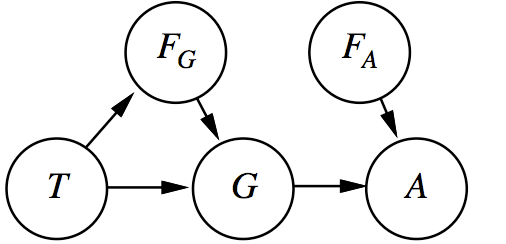
\includegraphics[width=\textwidth]{./images/nuclearpowerstationbayesiannet.png}
			\end{answer}
			\item Suppose there are just two possible actual and measured temperatures, normal and high, and the probability that the gauge gives the correct temperature is $x$ when it is working, but $y$ when it is faulty. Give the conditional probability table associated with node $G$.
			\marks{5}
			\begin{answer}
			Note the semantics of $F_G$ , which is true when the gauge is faulty, i.e., not working.
			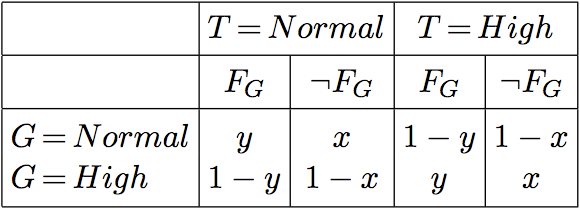
\includegraphics[width=\textwidth]{./images/cpt_node_g_q142.png}
			\end{answer}
			\item Suppose the alarm works correctly unless it is faulty, in which case it never sounds. Give the conditional probability table associated with A.
			\marks{5}
			\begin{answer}
			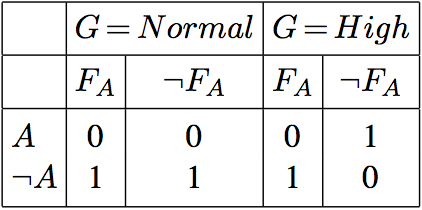
\includegraphics[width=\textwidth]{./images/cpt_a_q142.png}
			\end{answer}	
			%\item I have left out the rest of this question fill it in when I get a chance - the CPTs for part 2 and 3 are in the images folder.
		\end{enumerate}
		\item Consider the following time keeping patterns of the lecturers in your college:
			\begin{itemize}
				\item 25\% of lecturers start 75\% of their lectures on time and 25\% late.
				\item 50\% of lecturers start 50\% of their lectures on time and 50\% late.
						\item 25\% of lecturers start 25\% of their lectures on time and 75\% late.
			\end{itemize}
			\begin{enumerate}
				\item Given that both the $1^{st}$ and $2^{nd}$ Artificial Intelligence lectures of the year started on time, compute the posterior probability that your Artificial Intelligence lecturer follows that each of the three time-keeping patterns.
				\marks{5}
				\begin{answer}
					To begin we will define some notation. Let: 
					\begin{itemize}
						   \item $h_1$ denote the hypothesis that your AI lecturer starts 75\% of their lectures on time $P(h_1)=0.25$.
						   \item $h_2$ denote the hypothesis that your AI lecturer starts 50\% of their lectures on time $P(h_2)=0.50$.
			   						   \item $h_3$ denote the hypothesis that your AI lecturer starts 25\% of their lectures on time $P(h_3)=0.25$.
					\end{itemize}
					Also, if we use the notation $ontime_x$ to represent the observation that a lecture x started on time, then the probability of any given AI lecture starting on time given a particular hypothesis $h$ is:
					\begin{itemize}
						\item $P(ontime_x|h_1)=0.75$ .
						\item $P(ontime_x|h_2)=0.50$ .
						\item $P(ontime_x|h_3)=0.25$ .
					\end{itemize}
					Then:
						\begin{itemize}
							\item By Bayes' rule, we can compute the posterior probability of a hypothesis given the data so far using: 
											\begin{center}
											$P(h_i|\textbf{d}) = \alpha P(\textbf{d}|h_i) P(h_i)$
											\end{center}
				      		\item And, the likelihood of the data given a hypothesis is calculated using: 
											\begin{center}
											$P(\textbf{d}|h_i) = \prod_j P(d_j|h_i)$
											\end{center}
				           \end{itemize}
				       So:
				\begin{itemize}
					\item $P(h_1|ontime_1,ontime_2)=\alpha (\prod_{j=1}^2 P(ontime_j|h_1))P(h_1)=\alpha 0.75^2 \times 0.25=\alpha 0.375=\frac{0.375}{1.0} = 0.375$.
					\item $P(h_2|ontime_1,ontime_2)=\alpha (\prod_{j=1}^2 P(ontime_j|h_2))P(h_1)=\alpha 0.50^2 \times 0.50=\alpha 0.500=\frac{0.500}{1.0} = 0.500$.
					\item $P(h_3|ontime_1,ontime_2)=\alpha (\prod_{j=1}^2 P(ontime_j|h_3))P(h_1)=\alpha 0.25^2 \times 0.25=\alpha 0.125=\frac{0.125}{1.0} = 0.125$.
				\end{itemize}
			\end{answer}
				\item Given that both the $1^{st}$ and $2^{nd}$ Artificial Intelligence lectures of the year started on time, what is the Bayesian Prediction that the $3^{rd}$ Artificial Intelligence lecture will start on time? 
							   \marks{5}
					\begin{answer}
								Bayesian predictions use a likelihood-weighted sum over the hypotheses: 
								\begin{center}
								$P(X|\textbf{d})=\sum_i P(X|h_i)P(h_i|\textbf{d})$
								\end{center}
							     In this instance we get:
							     						\begin{eqnarray*}
P(ontime_{3}|\textbf{d})&=&\sum_i P(ontime_{3}|h_i)P(h_i|\textbf{d})\\
&=& (0.75 * 0.375) + (0.5 * 0.5) + (0.25 *0.125)\\
&=& 0.28125 + 0.25 + 0.03125\\
&=& 0.5625			
	\end{eqnarray*}
					\end{answer}
						\item Given that both the $1^{st}$ and $2^{nd}$ Artificial Intelligence lectures of the year started on time, what is the Maximum a Posterior (MAP) probability that the $3^{rd}$ Artificial Intelligence lecture will start on time? 
							   \marks{5}
				         \begin{answer}
				         A MAP prediction just uses the prediction provided by the single most probable hypothesis. From part one of the question we can see that given that both the $1^{st}$ and $2^{nd}$ lectures started on time the single most probable hypothesis is the hypothesis that the Artificial Intelligence lecturer will start 50\%  of their lectures on time (from part 1, $(P(h_2|ontime_1,ontime_2) = 0.5) > (P(h_2|ontime_1,ontime_2)=0.375) > (P(h_3|ontime_1,ontime_2)=0.125)$. This hypothesis would predict that the $3^{rd}$ AI lecture will start on time with a probability of $0.5$.
				         \end{answer}
			\end{enumerate}
\end{enumerate}

\newpage

%Q3
%Inductive Learning (Decision Trees)
%aima chapters 18
% learning theory - supervised/unsupervised, overfitting, lazy/eager learner, classification v regression, false positive v false negatives, linear separability, consistency
% decision trees (entropy)
% knn
\question
\begin{enumerate}
\item Define what is meant by \textbf{lazy learners} and \textbf{eager learners}, highlight the key differences between these approaches \textbf{and} give an example of each.
	\marks{10}
		\begin{answer}
			Definitions:
			\begin{description}
				\item [Lazy learners] do not try to build a model from the training data, but simply use it at classification time
				\item [Eager learners] build a mode from the training data during training, and use only this model at classification time, ignoring the original data.
			\end{description}
			Key differences:
			\begin{itemize}
				\item Lazy methods may consider query instance when deciding how to generalise beyond the training data D; eager methods cannot since they have already chosen global approximation when seeing the query.
				\item \textbf{Efficiency} lazy learners require less training times but more time at prediction; eager learners require more training times by less time for prediction
				\item \textbf{Accuracy} lazy learners effectively uses a richer hypothesis space since it uses many local linear functions to form its implicit global approximation to the target function; eager learners must commit to a single hypothesis that covers the entire instance space.
				\item It is easier for lazy learners to handle \textbf{concept drift}
			\end{itemize}
			Examples:
			\begin{description}
				\item [Lazy learning example]: case based reasoning
				\item [Eager learning example]: Decision=tree, neural networks, support vector machines
			\end{description}
		\end{answer}
	
%10 marks for decision trees
\item Formally define what is meant by the term \textbf{entropy} in the context of Decision Tree Learning.
		\marks{5}
	\begin{answer}
	For $c$ classification categories the entropy $E$ is defined as: $E=\sum_{i=1}^{c} -p_i\ log_2\ p_i$ where $p_i$ is the probability of category $i$ occurring.
	\end{answer}

\begin{table}[htdp]
\caption{The attributes of a newly discovered animal. A 1 indicates the animal possesses the feature listed in the column and 0 indicates that they do not. The column on the right contains a ? because the animal has not been classified yet.}
\begin{center}
\begin{tabular}{|c|c|c|c|c|c|c|c|c|c|c|}
\hline
Species & \begin{sideways}Births Live Young\end{sideways} & \begin{sideways}Lays Eggs\end{sideways} & \begin{sideways}Feeds Offspring Own Milk\end{sideways} & \begin{sideways}Warm-Blooded\end{sideways}  & \begin{sideways}Cold-Blooded \end{sideways} & \begin{sideways}Lives in Water and Land \end{sideways} & \begin{sideways}Has Hair \end{sideways} & \begin{sideways}Has Feathers\end{sideways} & Class \\
\hline 
Mystery & 0 & 1 & 0 & 0 & 0 & 1 & 0 & 0 & ? \\
\hline
\end{tabular}
\end{center}
\label{tab:animal-attributes}
\end{table}%

\begin{table}[htdp]
\caption{Example feature vectors for animal classification. A 1 indicates the animal possesses the feature listed in the column and 0 indicates that they do not. The rightmost column lists the classification of each ainmal.}
\begin{center}
\begin{tabular}{|c|c|c|c|c|c|c|c|c|c|c|}
\hline
Species & \begin{sideways}Births Live Young\end{sideways} & \begin{sideways}Lays Eggs\end{sideways} & \begin{sideways}Feeds Offspring Own Milk\end{sideways} & \begin{sideways}Warm-Blooded\end{sideways}  & \begin{sideways}Cold-Blooded \end{sideways} & \begin{sideways}Lives in Water and Land \end{sideways} & \begin{sideways}Has Hair \end{sideways} & \begin{sideways}Has Feathers\end{sideways} & Class \\
\hline 
Cat & 1 & 0 & 1 & 1 & 0 & 0 & 1 & 0 & Mammal \\
Frog & 0 & 1 & 0 & 0 & 1 & 1 & 0 & 0 & Amphibian \\
Squirrel & 1 & 0 & 1 & 1 & 0 & 0 & 1 & 0 & Mammal \\
Duck & 0 & 1 & 0 & 1 & 0 & 1 & 0 & 1 & Bird \\
\hline
\end{tabular}
\end{center}
\label{tab:ainmals-classification}
\end{table}%
		
\item You are working as an assistant-biologist to Charles Darwin on the Beagle voyage. You are at the Gal\'apagos Islands and you have just discovered a new animal that has not yet been classified. Table \ref{tab:animal-attributes} lists the attributes of the animal you have found. Mr. Darwin has asked you to classify the animal using a nearest-neighbour approach and he has supplied you with a case-base of already classified animals, see Table \ref{tab:ainmals-classification}. 
\begin{enumerate}
\item A good measure of distance between two instances with categorical features is the number of features which have different values (the \textbf{overlap metric}, also known as the \textbf{hamming distance}). Using this measure of distance compute the distance between the mystery animal and each of the animals in the case base. 
	\marks{5}
	\begin{answer}
	\begin{center}
\begin{tabular}{|c|c|c|}
\hline
Species & Class & Distance\\
\hline 
Cat & Mammal & 6\\
Frog & Amphibian & 1\\
Squirrel & Mammal & 6\\
Duck & Bird & 2\\
\hline
\end{tabular}
	\end{center}
	\end{answer}
\item If you used $1-NN$ classification what class would be assigned to the mystery animal.
	\marks{5}
	\begin{answer}
	The nearest neighbor to the mystery animal is the Frog. So the mystery animal would be classified as an amphibian.
	\end{answer}
\item If the you used $4-NN$ classification what class would be assigned to the mystery animal. 
	\marks{5}
	\begin{answer}
	If you applied a $4-NN$ classification to this case-base you would include all the instances in the case-base irrespective of their distance from the test instance feature vector. As a result the test instance would be assigned the most frequently occurring class in the case-base. This would result in the mystery animal being classified as a mammal. 
	\end{answer}
\end{enumerate}

\end{enumerate}

\newpage

%Q4
%Linear Regression Neural Nets, SVMs, Ensemble Learning
%Inductive Logic programming
\question 
	\begin{enumerate}
		\item Figure \ref{fig:mystery-perceptron}, on the next page, is a schematic of a 3 input perceptron. Input $a_0 = -1$, inputs $a_1$ and $a_2$ are binary. The perceptron uses a threshold activation function that outputs a 1 if the weighted sum of inputs is greater than 0 and a 0 otherwise. Define the truth-table of the function that this perceptron implements and identify the name of the function. 
		\marks{5}
		\begin{answer}
		   {\Large
   \begin{tabular}{@{} ccc | c | c @{}}
      \multicolumn{3}{c}{Inputs} & $in_i$ & $a_i$ \\ \hline
      $a_0$ & $a_1$ & $a_2$ & $\sum_{j=0}^{2} w{j}{i} a_j$ & $\left( in_i  > 0\right)?(1):(0)$\\ \hline
      -1 & 1 & 1 & 0.5 & 1\\
      -1 & 1 & 0 & -0.5 & 0\\
      -1 & 0 & 1 & -0.5 & 0\\
      -1 & 0 & 0 & -1.5 & 0\\ \hline        
   \end{tabular}
   }\\
This perceptron implements the AND function.
		\end{answer}

\item Describe the perceptron training rule?
\marks{10}
	\begin{answer}
	Perceptrons learn by modifying the weights associated with their inputs. Consequently, the learning problem faced by perceptron training is to determine a weight vector that causes the perceptron to produce the correct $+-1$ output for each of the given training examples.

One way to learn an acceptable weight vector is to begin with random weights, then iteratively apply the perceptron to each training example, modifying the perceptron weights whenever it misclassifies an example.

Weights are modified at each step according to the \emph{perceptron training rule}, which revises the weight $w_i$ associated with input $a_i$ according to the rule:
\begin{center}
$w_i \leftarrow w_i + \Delta w_i$
\end{center}
where
\begin{center}
$\Delta w_i = \eta(t - o) a_i$
\end{center}

where t = target output, o = observed output, $\eta$ is a positive constant called the \emph{learning rate}. The role of the learning rate is to moderate the degree to which weights are changed at each step. It is usually set to some small value (e.g.$0.1$) and is sometimes made to decay as the number of weight-training iterations increases.
\end{answer}

\item Why does the perceptron training rule converge toward successful weight values?
\marks{5}
\begin{answer}
If the training example is \emph{correctly classified} $(t-o)=0 \rightarrow \Delta w_i =0$ so \emph{no weights are updated}.

If the case of a \emph{false negative} (o=0 and t=1) we want to make the perceptron output a 1 instead of a 0 so the weights must be altered to increase the value of $\vec{w} \bullet \vec{a}$. Notice that in this case \emph{the rule will increase $w_i$} because $(t-o), \eta$ and $a_i$ are all positive.

On the other hand, in the case of a \emph{false positive} (o=1 and t=0) then \emph{the weights associated with $a_i$ will be decreased}.
\end{answer}
	
	
	
	\item The FOIL inductive logic programming algorithm is constructing a new rule with head $p(Y) \leftarrow$. Which of the following literals could be considered as candidate extensions $q(Y)$, $r(X)$, $s(X,Y)$, $\lnot s(X,Y)$?
	\marks{5}
\begin{answer}
Three of the given literals could be considered as extensions: $q(Y)$, $s(X,Y)$, $\lnot s(X,Y)$. The literal $r(X)$ would not be considered as an extension as it does not contain at least one variable that is already present in the rule.
\end{answer} 
	\item The FOIL inductive logic programming algorithm is considering adding a literal $l$ to a rule $r$. The extension of the rule $r$ before adding $l$ is the following set of positive and negative examples $\{+,+,+,+,+,+,-,-,-,- \}$. The extension of the rule after the literal is added (i.e. the extension of $r+l$) is $\{+,+,+,+,+,+,-,- \}$. What is the information gain of adding the literal $l$ to the rule $r$? (Note you do not need to calculate the logs in your answer (i.e. you can express your answer as an equation containing logs)).
	\marks{5}
\begin{answer}

\[Foil\_Gain(L,R) \equiv t \left( \log_{2}\frac{p_{1}}{p_{1}+n_{1}} -
\log_{2}\frac{p_{0}}{p_{0}+n_{0}} \right) \]

Where
\begin{itemize}
\item $L$ is the candidate literal to add to rule $R$
\item $p_0$ = number of positive bindings of $R$
\item $n_0$ = number of negative bindings of $R$
\item $p_1$ = number of positive bindings of $R+L$
\item $n_1$ = number of negative bindings of $R+L$
\item $t$ is the number of positive bindings of $R$ also covered by $R+L$
\end{itemize}

In this instance
\begin{itemize}
\item $p_0$ = 6
\item $n_0$ = 4
\item $p_1$ = 6
\item $n_1$ = 2
\item $t$ = 6
\end{itemize}

\[Foil\_Gain(L,R) \equiv 6 \left( \log_{2}\frac{6}{6+4} -
\log_{2}\frac{6}{6+2} \right) \]

\end{answer}

\end{enumerate}

\begin{figure}
 		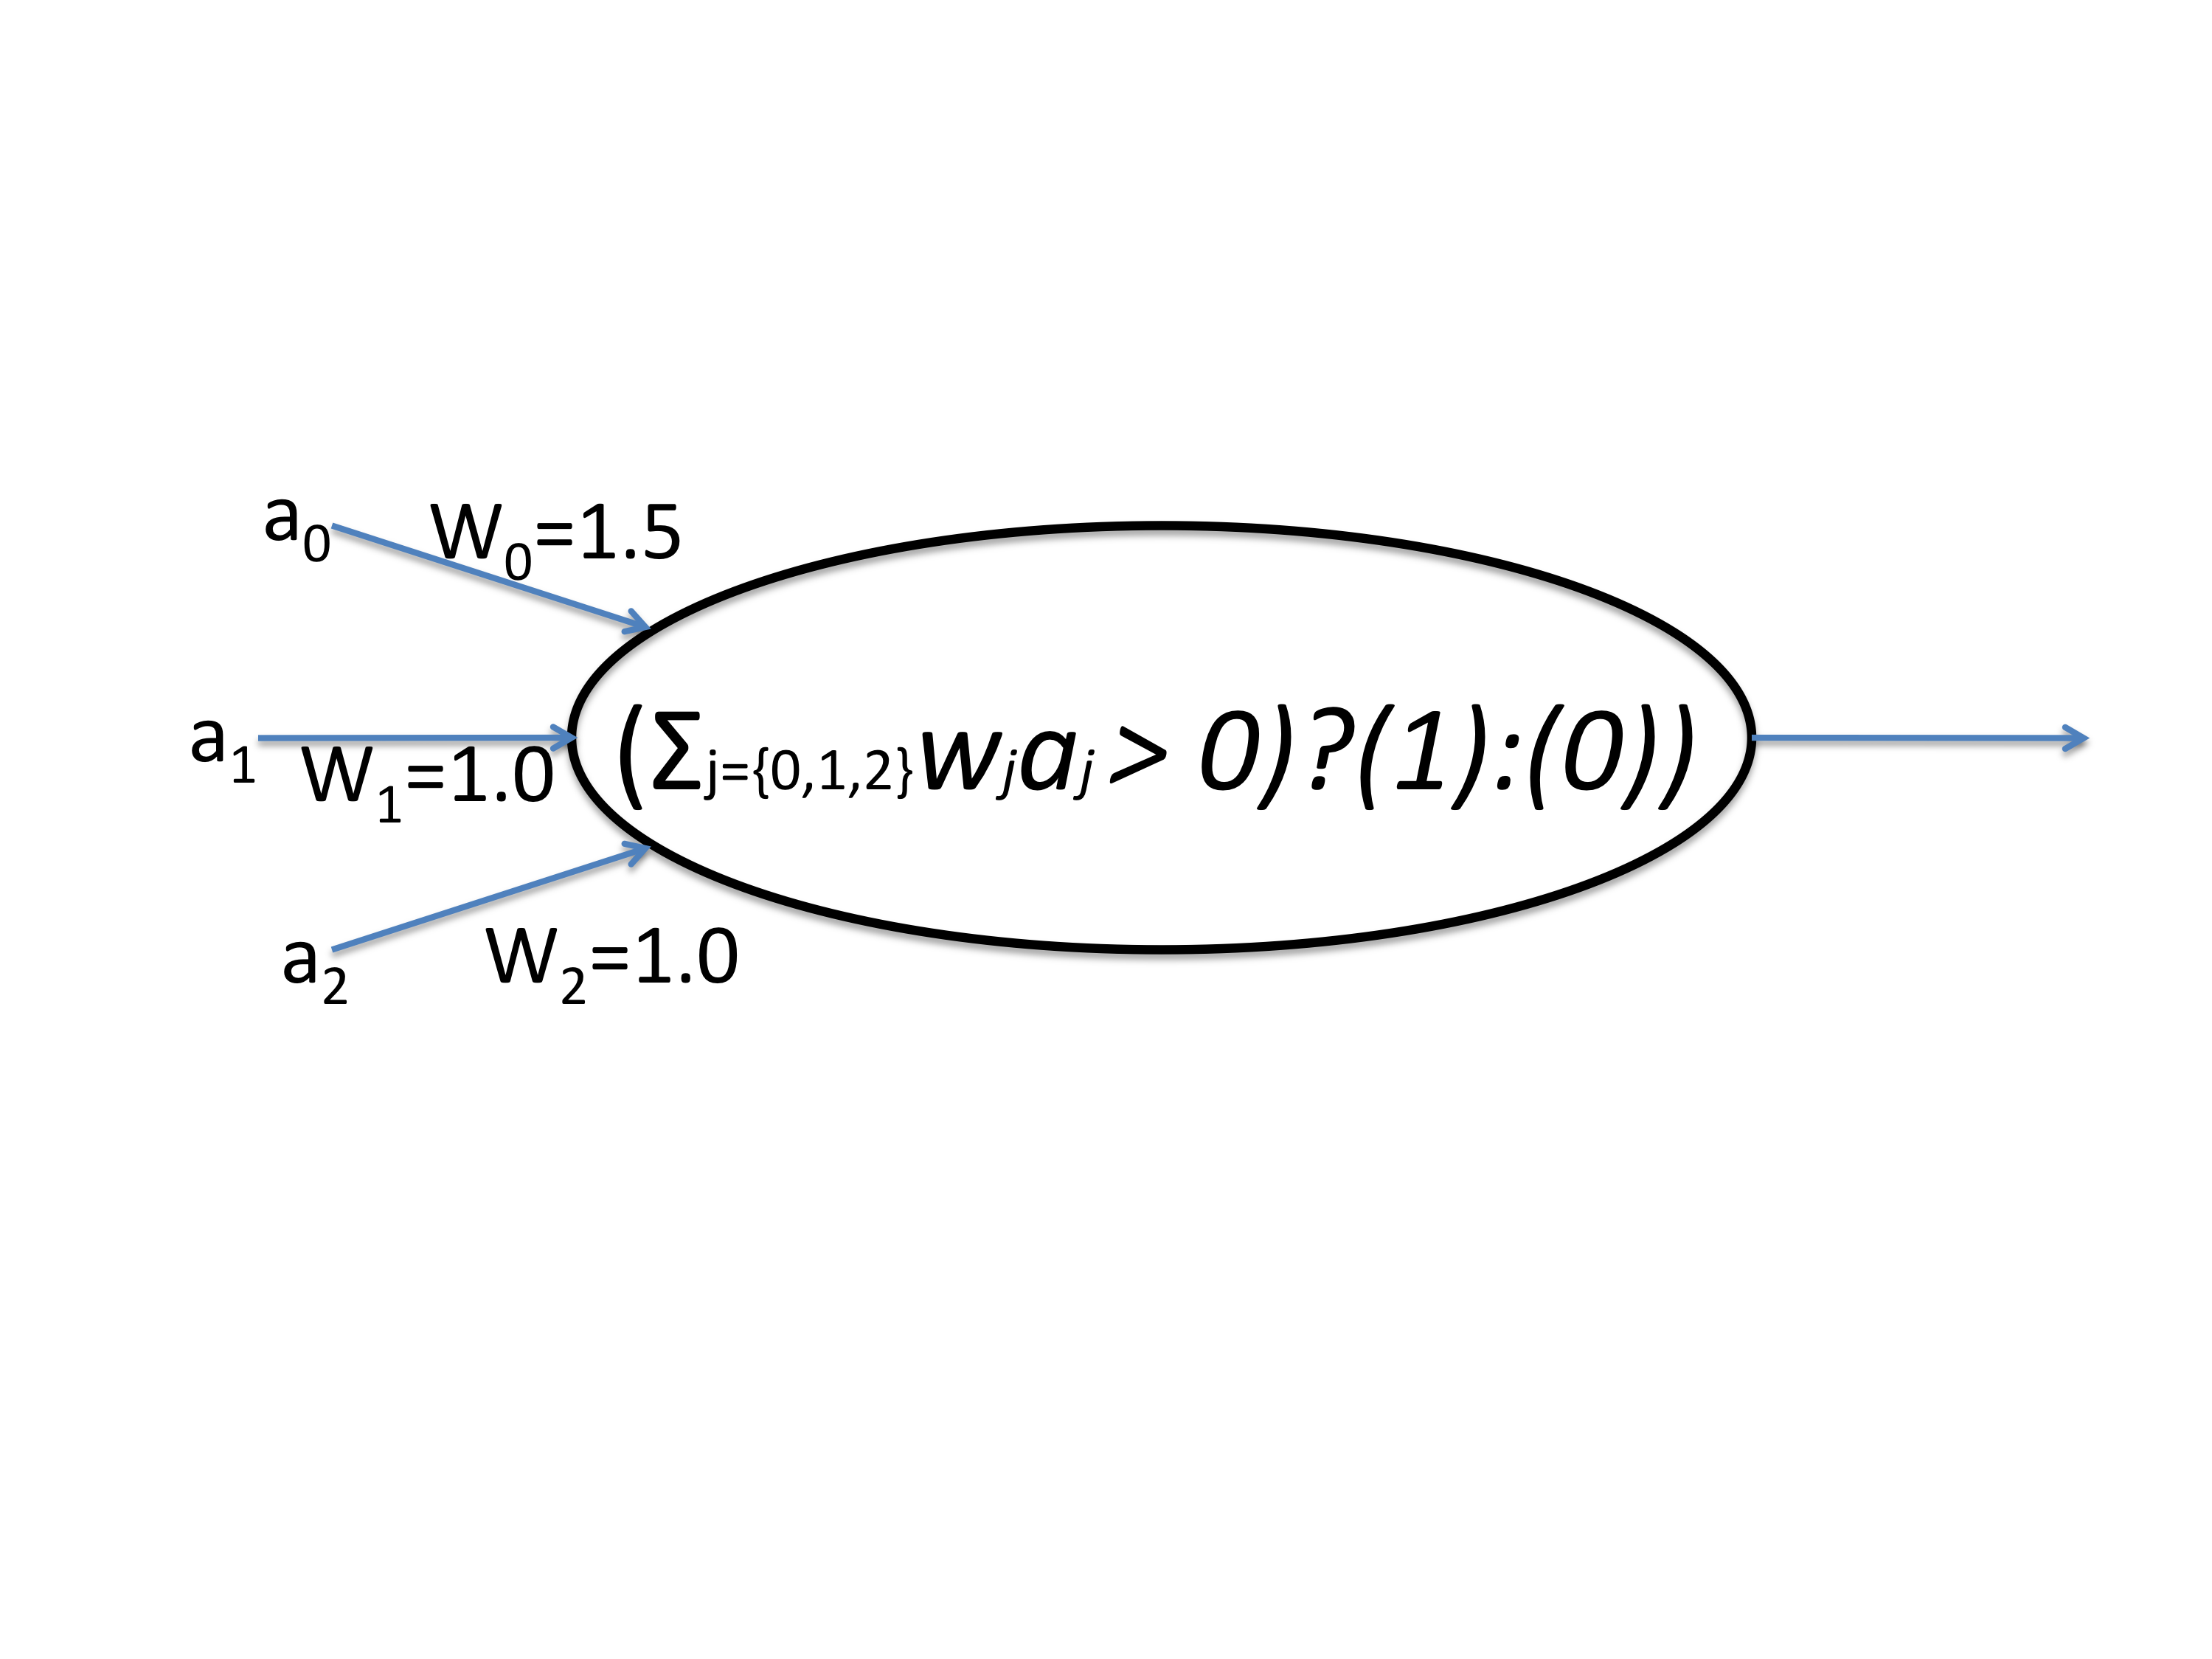
\includegraphics[width=4in]{./images/mystery-perceptron.png}
		\caption{A 3 input perceptron. Input $a_0 = -1$, inputs $a_1$ and $a_2$ are binary. The perceptron uses a threshold activation function that outputs a 1 if the weighted sum of inputs is greater than 0 and a 0 otherwise.}
		\label{fig:mystery-perceptron}
\end{figure}



\end{document}
